\documentclass[13.1pt, letterpaper, twoside]{article}
\usepackage[left=1.7cm,top=1.7cm, right=1.7cm,bottom=1.7cm]{geometry}
\usepackage[utf8]{inputenc}
\usepackage{enumerate}
\usepackage{enumitem}
\usepackage{bm}
\usepackage{parskip}
\usepackage{svg}
\usepackage{physics}
\usepackage{amsmath}
\usepackage{tikz}
\usepackage{mathdots}
\usepackage{yhmath}
\usepackage{cancel}
\usepackage{color}
\usepackage{siunitx}
\usepackage{lscape}
\usepackage{array}
\usepackage{multirow}
\usepackage{amssymb}
\usepackage{gensymb}
\usepackage{tabularx}
\usepackage{booktabs}
\usepackage{float}
\usepackage{graphicx}
\usepackage{subcaption}
\usepackage{setspace}
\usepackage{flushend}
\usepackage{multicol}
\usepackage{esvect}
\usepackage{fancyhdr}
\usepackage{xcolor}
\usepackage{soul}
\usepackage{booktabs}
\usepackage{tabularx}
\usepackage{amsmath,amssymb,bm}
\usepackage{slashed}
\usepackage[compat=1.1.0]{tikz-feynman}
\usepackage[colorlinks=true, allcolors=purple]{hyperref}
\usepackage[justification=centering]{caption}

\graphicspath{{figures/}}

\setlength{\parindent}{10pt}
\setlength{\columnsep}{25pt}
\pagestyle{fancy}
    \lhead[{\thepage}]{\emph{\small{The Sun as a Source of Excited States of Dark Matter}}} 
\rhead[D. Tinoco Villalba]{\thepage}
\cfoot{}
%\newcommand{\pp}[1][2][3]{\mathbb{#1}}
\newcommand{\pp}[3]{\left(\frac{\partial #1}{\partial #2}\right)_{#3}}
\renewcommand{\headrulewidth}{0pt}
\newcolumntype{P}[1]{>{\centering\arraybackslash}p{#1}}
\def\dbar{{\mkern3mu\mathchar'26\mkern-12mu d}}

\begin{document}

\thispagestyle{plain}

\begin{center}
	\textbf{\huge{Inelastic Solar Reflection of Dark Matter}}\\
	\vspace{6mm}
	\textbf{D. Tinoco Villalba}\\
	\vspace{3mm}
	\textbf{Professor: Harikrishnan Ramani}\\
	\vspace{6mm}
	\textbf{Department of Physics and Astronomy}\\
	\vspace{2mm}
	\textbf{University of Delaware, Newark, DE}\\
\end{center}

\section{Cross sections of inelastic processes}

\subsection{$\chi e \to \chi^\ast e$ scattering}

\subsubsection{Relativistic expression}

We start from the Lagrangian
\[
\mathcal{L}_{\text{int}}
= i\,\bar{\chi^\ast} \gamma^\mu D_\mu \chi
+ i\,\bar{e}\,\gamma^\mu D_\mu e
+ i\,\bar{N}\,\gamma^\mu D_\mu N
\]

\[
D_\mu=\partial_\mu-i g_v A^\mu
\]

For this process we only have to consider the t-channel 
\begin{center}
    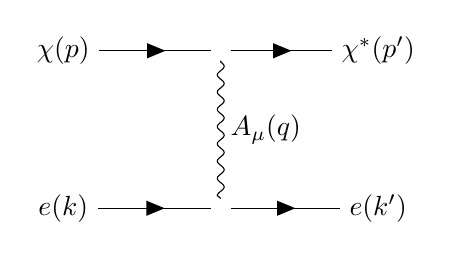
\begin{tikzpicture}
        \begin{feynman}
            \vertex (i1) at (-2, 1) {$\chi(p)$};
            \vertex (v1) at ( 0, 1) {};
            \vertex (o1) at ( 2, 1) {$\chi^\ast(p')$};

            \vertex (i2) at (-2,-1) {$e(k)$};
            \vertex (v2) at ( 0,-1) {};
            \vertex (o2) at ( 2,-1) {$e(k')$};

            \diagram*{
                (i1) -- [fermion] (v1) -- [fermion] (o1),
                (i2) -- [fermion] (v2) -- [fermion] (o2),
                (v1) -- [boson, edge label=$A_\mu(q)$] (v2),
            };
        \end{feynman}
    \end{tikzpicture}
\end{center}

\[
    \mathcal{M}
    = g_\chi g_e\, J_\chi^\mu \left[\frac{g_{\mu\nu}}{q^2-m_{A'}^2}\right] J_e^\nu
    = \,\frac{g_\chi g_e}{q^2-m_{A'}^2}\,
    \big[\bar{u}_{\chi^\ast}(p')\gamma^\mu u_\chi(p)\big]
        \big[\bar{u}_e(k')\gamma_\mu u_e(p)\big]
\]

And, averaging over the spins
\[
    \sum_{\text{spins}} \lvert \mathcal{M}\rvert^2
    = \frac{(g_\chi g_e)^2}{(q^2-m_{A'}^2)^2} \sum_{s,s'}\;
    \big[\bar{u}_{\chi^\ast s'}(p')\gamma^\mu u_{\chi s}(p)\big]
        \big[\bar{u}_e(k')\gamma_\mu u_e(k)\big]
        \big[\bar{u}_e(k')\gamma_\nu u_e(k)\big]^{*}
        \big[\bar{u}_{\chi^\ast s'}(p')\gamma^\nu u_{\chi s}(p)\big]^{*}
\]

\[
    = -\,\frac{(g_\chi g_e)^2}{(q^2-m_{A'}^2)^2} \sum_{s,s'}\;
    \big[\bar{u}_{\chi^\ast s'}(p')\gamma^\mu u_{\chi s}(p)\big]
        \big[\bar{u}_e(k')\gamma_\mu u_e(k)\big]
    \big[\bar{u}_e(k)\gamma_\nu u_e(k')\big]
    \big[\bar{u}_{\chi s}(p)\gamma^\nu u_{\chi^\ast s'}(p')\big]
\]

Remembering the relation
\[
\sum_s u(p,s)\,\bar{u}(p,s) \;=\; \slashed{p} + m
\]

We have
\[
\sum_{\text{spins}} |\mathcal{M}|^2
= \frac{(g_\chi g_e)^2}{(q^2 - m_{A'}^2)^2}\,
\mathrm{Tr}\!\left[(\slashed{p}' + m_\chi)\gamma^\mu(\slashed{p}+m_\chi)\gamma^\nu\right]\,
\mathrm{Tr}\!\left[(\slashed{k}' + m_e)\gamma_\mu(\slashed{k}+m_e)\gamma_\nu\right]
\]

And using the identity
\[
\mathrm{Tr}\!\left[(\slashed{a}+m)\gamma^\mu(\slashed{b}+m)\gamma^\nu\right]
= 4\left(a^\mu b^\nu + a^\nu b^\mu - g^{\mu\nu}(a\cdot b - m^2)\right)
\]

We obtain
\[
\sum_{\text{spins}} |\mathcal{M}|^2
= \frac{16\,(g_\chi g_e)^2}{(q^2 - m_{A'}^2)^2}\,
\Big[p'^\mu p^\nu + p'^\nu p^\mu - g^{\mu\nu}(p'\cdot p - m_\chi^2)\Big]\,
\Big[k'_\mu k_\nu + k'_\nu k_\mu - g_{\mu\nu}(k'\cdot k - m_e^2)\Big]
\]

Contracting the products and reordering terms, we reach the invariant expression for the amplitude:
\begin{equation}
    \overline{|\mathcal{M}|^2}
    = \frac{1}{4\ \text{spins}} \sum |\mathcal{M}|^2
    = \frac{8\,(g_\chi g_e)^2}{(q^2 - m_{A'}^2)^2}
    \Big[ (p'\!\cdot k')(p\!\cdot k) + (p'\!\cdot k)(p\!\cdot k') - m_e^2 (p'\!\cdot p) - m_\chi m_{\chi^\ast} (k'\!\cdot k) + 2 m_e m_\chi m_{\chi^\ast} \Big]    
    \label{invamplitude}
\end{equation}

In the lab frame, choosing the $x-z$ plane as the scattering plane,
\[
p = (E_\chi, 0, 0, |\vec{p}|), 
\qquad |\vec{p}| = \sqrt{E_\chi^2 - m_\chi^2}
\]

\[
k = (m_e, \vec{0}),
\qquad |\vec{k}| = \sqrt{E_R(E_R + 2 m_e)}
\]

\[
k' = (m_e + E_R,\, |\vec{k}'|\sin\theta_e,\, 0,\, |\vec{k}'|\cos\theta_e)
\]

\[
p' = (E_\chi - E_R,\,-|\vec{k}'|\sin\theta_e,\, 0,\, |\vec{p}| - |\vec{k}'|\cos\theta_e)
\]

\[
q^2 = (k - k')^2 = |\vec{k}|^2 - |\vec{k}'|^2 
= -E_R^2 - E_R(E_R + 2 m_e) = -2 m_e E_R
\]

with $E_R$ the electron recoil energy and $\theta_e$ the scattering angle.  
From $p'^2 = m_{\chi^\ast}^2$ we get
\[
\cos\theta_e 
= \frac{m_{\chi^\ast}^2 - m_\chi^2 + 2E_R(m_e + E_\chi)}{2|\vec{p}||\vec{k}'|}
\]

Then 

\[
p \cdot k = m_e E_\chi, 
\qquad 
p' \cdot k = m_e(E_\chi - E_R)
\]

\[
p \cdot k' = m_e E_\chi - m_e E_R + \tfrac{1}{2}\left(m_\chi^2 - m_{\chi^\ast}^2\right)
\]

\[
p' \cdot k' = m_e E_\chi + \tfrac{1}{2}\left(m_\chi^2 - m_{\chi^\ast}^2\right)
\]

\[
k \cdot k' = m_e(m_e + E_R),
\qquad
p \cdot p' = \tfrac{1}{2}\left(m_\chi^2 + m_{\chi^\ast}^2\right) + m_e E_R
\]

Replacing all the scalar products in \ref{invamplitude} and grouping similar terms, we obtain
\begin{gather*}
    \overline{|\mathcal{M}|^2} = \frac{8\,(g_\chi g_e)^2}{(q^2 - m_{A'}^2)^2}\, m_e 
    \Bigg[
    2 m_e E_\chi^2 + E_\chi m_\chi^2 
    - 2 m_e E_\chi E_R + m_e E_R^2
    - \tfrac{1}{2} E_R m_\chi^2 - m_e^2 E_R 
    - \tfrac{1}{2} m_e m_\chi^2  
    + m_\chi (m_e - E_R)m_{\chi^\ast} \\
    + \tfrac{1}{2}(E_R - m_e - 2E_\chi)m_{\chi^\ast}^2
    \Bigg]    
\end{gather*}

And substituting $m_{\chi^\ast} = m_x + \delta$, we get
\[
\overline{|\mathcal{M}|^2} = \frac{8\,(g_\chi g_e)^2}{(q^2 - m_{A'}^2)^2}\, m_e
\Bigg[
  2 m_e E_\chi^2
  - (2 m_e E_\chi + m_e^2 + m_\chi^2) E_R
  + m_e E_R^2
  - 2 m_\chi E_\chi \,\delta
  + \tfrac{1}{2}\,(E_R - 2E_\chi - m_e)\,\delta^2
\Bigg]
\]

The cross section is given by
\[
\frac{d\sigma}{dE_R} 
= \frac{dq^2}{dE_R}\,\frac{d\sigma}{dq^2}
= 2 m_e \left( \frac{|\overline{\mathcal{M}}|^2}{64\pi m_e^2 |\vec{p}|^2} \right)
= \frac{|\overline{\mathcal{M}}|^2}{32\pi m_e (E_\chi^2 - m_\chi^2)} 
\]

with 
\[
q^2 = (k - k')^2 = -E_R^2 - |\vec{k}'|^2 \sin^2\theta_e - |\vec{k}'|^2 \cos^2\theta_e
= E_R^2 - E_R^2 - 2 m_e E_R 
\]

Considering that
\[
\big(q^2 - m_{A'}^2\big)^2 = \big(-2 m_e E_R - m_{A'}^2\big)^2
= \big(m_{A'}^2 + 2 m_e E_R\big)^2 
\]

We finally obtain

\subsubsection{NR limit}

\subsection{$\chi N \to \chi^\ast N$ scattering}

\section{Flux of $\chi^{\ast}$}

\subsection{Up-scattered by electrons}

Inside the Sun we treat the incoming dark matter (DM) as essentially at rest while thermal electrons upscatter it to the excited state \(\chi^\ast\).
Gravitational focusing enhances the steady--state DM density in the core; to the accuracy used in the paper one takes
\[
n_{\chi,\odot}\simeq n_0\,\frac{v_{\rm esc}}{v_0},\qquad
n_0=\frac{\rho_\chi}{m_\chi},
\]
with \(v_{\rm esc}\simeq 1500~\mathrm{km\,s^{-1}}\) and \(v_0\simeq 220~\mathrm{km\,s^{-1}}\).
The flux of \(\chi^\ast\) at Earth is then
\[
\;
\Phi \;=\; n_e\,\big\langle\sigma_{\chi\to\chi^\ast}\,v_e\big\rangle\;
\frac{n_{\chi,\odot}\,V_\odot}{4\pi\,(1~\mathrm{AU})^2
\;},
\]
and the differential flux per outgoing \(\chi^\ast\) kinetic energy,
\begin{equation}
    \boxed{\;
    \frac{d\Phi}{dK_{\chi^\ast}}
    \;=\; n_e\,
    \Big\langle \frac{d\sigma_{\chi\to\chi^\ast}}{dK_{\chi^\ast}}\,v_e\Big\rangle
    \frac{n_{\chi,\odot}\,V_\odot}{4\pi\,(1~\mathrm{AU})^2}\,}\; ,
    \label{fluxdiff}
\end{equation}

with \(T_\odot\simeq 1.1~\mathrm{keV}\), \(n_e\simeq 2\times 10^{25}~\mathrm{cm^{-3}}\), and \(V_\odot\simeq 2.2\times 10^{31}~\mathrm{cm^3}\).

\smallskip
\noindent
In the nonrelativistic (NR) limit used in the paper (heavy/contact mediator and \(\delta\ll m_e,m_\chi\)), the differential upscattering cross section is taken as
\[
\;
\frac{d\sigma_{\chi\to\chi^\ast}}{dK_{\chi^\ast}}
=\frac{\overline{\sigma}_e\,m_\chi}{2\,\mu_{\chi e}^2\,v_e^{\,2}}\,,\qquad
\mu_{\chi e}=\frac{m_\chi m_e}{m_\chi+m_e}\,,
\;
\]
and the thermal average entering is performed over a Maxwell--Boltzmann (MB) speed distribution
\[
\;
f_{\rm MB}(v_e)=4\pi v_e^2\left(\frac{m_e}{2\pi T_\odot}\right)^{\!\!3/2}
\exp\!\left[-\,\frac{m_e v_e^2}{2T_\odot}\right],
\;
\]
with a kinematic threshold on the electron speed at fixed \(K_{\chi^\ast}\),
\[
\;
v_{\min}(K_{\chi^\ast})=
\frac{1}{\sqrt{2m_\chi K_{\chi^\ast}}}\left(\frac{m_\chi K_{\chi^\ast}}{\mu_{\chi e}}+\delta\right),
\;
\]
Thus,
\[
\;
\Big\langle \frac{d\sigma}{dK_{\chi^\ast}}\,v_e\Big\rangle
=\int_{v_{\min}}^{\infty}\!\!dv_e\; f_{\rm MB}(v_e)\;
\frac{\sigma_e\,m_\chi}{2\,\mu_{\chi e}^2}\,\frac{1}{v_e}\,.
\;
\]

\noindent
Set \(a \equiv \dfrac{m_e}{2T_\odot}\).
Then
\[
\int_{v_{\min}}^{\infty}\!dv_e\;f_{\rm MB}(v_e)\,\frac{1}{v_e}
=4\pi\!\left(\frac{m_e}{2\pi T_\odot}\right)^{\!3/2}\!
\int_{v_{\min}}^{\infty}\!dv_e\; v_e\,e^{-a v_e^2}\; .
\]
Using \(\displaystyle \int v\,e^{-a v^2}\,dv = -\frac{1}{2a}e^{-a v^2}\) and
evaluating at the limits gives
\[
\int_{v_{\min}}^{\infty}\!dv_e\; v_e\,e^{-a v_e^2}
=\frac{1}{2a}\,e^{-a v_{\min}^2}
=\frac{T_\odot}{m_e}\,e^{-\frac{m_e v_{\min}^2}{2T_\odot}}.
\]
Therefore
\[
\int_{v_{\min}}^{\infty}\!dv_e\;f_{\rm MB}(v_e)\,\frac{1}{v_e}
=4\pi\!\left(\frac{m_e}{2\pi T_\odot}\right)^{\!3/2}
\frac{T_\odot}{m_e}\,e^{-\frac{m_e v_{\min}^2}{2T_\odot}}
=\sqrt{\frac{2}{\pi}}\;\sqrt{\frac{m_e}{T_\odot}}\;
e^{-\frac{m_e v_{\min}^2}{2T_\odot}} .
\]
Multiplying the overall factor \(\sigma_e m_\chi/(2\mu_{\chi e}^2)\) we obtain the analytic result
\begin{equation}
    \boxed{\;
    \Big\langle \frac{d\sigma}{dK_{\chi^\ast}}\,v_e \Big\rangle
    =\frac{\sigma_e\,m_\chi}{2\,\mu_{\chi e}^2}\;
    \sqrt{\frac{2}{\pi}}\;\sqrt{\frac{m_e}{T_\odot}}\;
    \exp\!\left[-\frac{m_e\,v_{\min}^2(K_{\chi^\ast})}{2T_\odot}\right]}\; .
    \label{avgdiffcrosssection}
\end{equation}

Now, to get the thermally–averaged rate, we also integrate over $K_{\chi^\ast}$,
\[
\big\langle \sigma_{\chi\to\chi^\ast} v_e \big\rangle
=\int_{0}^{\infty} dK\;
\Big\langle \frac{d\sigma}{dK}\,v_e \Big\rangle .
\]
We can write
\[
\exp\!\left[-\frac{m_e v_{\min}^2}{2T_\odot}\right]
=\exp\!\left[-\alpha\frac{\delta}{\mu_{\chi e}}\right]
\exp\!\left[-\beta K-\frac{\gamma}{K}\right],
\quad
\beta\equiv\alpha\frac{m_\chi}{2\mu_{\chi e}^2},\ \ 
\gamma\equiv\alpha\frac{\delta^2}{2m_\chi}.
\]
Hence
\[
\big\langle \sigma_{\chi\to\chi^\ast} v_e \big\rangle
=\frac{\bar\sigma_e\,m_\chi}{2\,\mu_{\chi e}^2}
\sqrt{\frac{2}{\pi}}\sqrt{\frac{m_e}{T_\odot}}
\;e^{-\alpha\delta/\mu_{\chi e}}
\int_{0}^{\infty} dK\; e^{-\beta K-\gamma/K}.
\]
Using the standard result
\[
\int_{0}^{\infty} dx\; e^{-\beta x-\gamma/x}
=2\sqrt{\frac{\gamma}{\beta}}\;K_{1}\!\left(2\sqrt{\beta\gamma}\right)
\qquad(\Re\beta,\Re\gamma>0),
\]
And considering that
\[
2\sqrt{\frac{\gamma}{\beta}}
=2\sqrt{ \frac{\alpha \delta^2}{2m_\chi}\cdot\frac{2\mu_{\chi e}^2}{\alpha m_\chi} }
=2\,\frac{\mu_{\chi e}\,\delta}{m_\chi},
\qquad
2\sqrt{\beta\gamma}
=2\sqrt{\frac{\alpha m_\chi}{2\mu_{\chi e}^2}\cdot\frac{\alpha\delta^2}{2m_\chi}}
=\alpha\,\frac{\delta}{\mu_{\chi e}},
\]
we obtain
\[
\boxed{\
\big\langle \sigma_{\chi\to\chi^\ast} v_e \big\rangle
=\bar\sigma_e\;
\sqrt{\frac{2m_e}{\pi T_\odot}}\;
\frac{\delta}{\mu_{\chi e}}\;
\exp\!\left(-\frac{m_e\delta}{2\mu_{\chi e}T_\odot}\right)
K_{1}\!\left(\frac{m_e\delta}{2\mu_{\chi e}T_\odot}\right) 
}\; .
\]

\noindent
\textbf{Asymptotics:}
Let $z\equiv x=\dfrac{m_e\delta}{2\mu_{\chi e}T_\odot}$.

\smallskip
\emph{Small splitting / hot plasma:}\; $z\ll1$.
For $\nu>0$, $K_\nu(z)\sim 2^{\nu-1}\Gamma(\nu)\,z^{-\nu}$; in particular
$K_1(z)\simeq 1/z$.
Then $e^{-z}K_1(z)\simeq 1/z$ and
\[
\big\langle \sigma v \big\rangle
\simeq \bar\sigma_e\sqrt{\frac{2m_e}{\pi T_\odot}}
\frac{\delta}{\mu_{\chi e}}\frac{1}{z}
=\bar\sigma_e\sqrt{\frac{2m_e}{\pi T_\odot}}
\frac{\delta}{\mu_{\chi e}}
\frac{2\mu_{\chi e}T_\odot}{m_e\delta}
=\ \bar\sigma_e\,\sqrt{\frac{8T_\odot}{\pi m_e}}\ .
\]

\smallskip
\emph{Large splitting / cool plasma:}\; $z\gg1$.
Use $K_\nu(z)\sim \sqrt{\dfrac{\pi}{2z}}\,e^{-z}\!\left[1+\dfrac{4\nu^2-1}{8z}+\cdots\right]$,
so $e^{-z}K_1(z)\simeq \sqrt{\dfrac{\pi}{2z}}\,e^{-2z}$.
Hence
\[
\big\langle \sigma v \big\rangle
\simeq \bar\sigma_e\sqrt{\frac{2m_e}{\pi T_\odot}}
\frac{\delta}{\mu_{\chi e}}
\sqrt{\frac{\pi}{2z}}\,e^{-2z}
=\bar\sigma_e\,\sqrt{\frac{2\delta}{\mu_{\chi e}}}\,
\exp\!\Big(-\frac{m_e\delta}{\mu_{\chi e}T_\odot}\Big).
\]
Thus
\[
\boxed{\
\big\langle \sigma_{\chi\to\chi^\ast} v_e \big\rangle
\simeq
\bar\sigma_e\!\times\!
\begin{cases}
\displaystyle \sqrt{\dfrac{8T_\odot}{\pi m_e}}, & \dfrac{\delta}{\mu_{\chi e}}\ll \dfrac{2T_\odot}{m_e},\\[10pt]
\displaystyle \sqrt{\dfrac{2\delta}{\mu_{\chi e}}}\;
\exp\!\Big(-\dfrac{m_e\delta}{\mu_{\chi e}T_\odot}\Big), &
\dfrac{\delta}{\mu_{\chi e}}\gg \dfrac{2T_\odot}{m_e}.
\end{cases}
}
\]

Replacing \ref{avgdiffcrosssection} in \ref{fluxdiff}, we get the complete expression for the differential flux of up-scattered $\chi^\ast$:
\[
\boxed{\frac{d\Phi}{dK_{\chi^\ast}}
= n_e\;
\frac{\sigma_e\, m_\chi}{2\,\mu_{\chi e}^2}\,
\sqrt{\frac{2}{\pi}}\sqrt{\frac{m_e}{T_\odot}}\,
\exp\!\left[-\frac{m_e\,v_{\min}^2(K_{\chi^\ast})}{2T_\odot}\right]\;
\frac{n_{\chi,\odot}\,V_\odot}{4\pi\,(1~\mathrm{AU})^2}}\, .
\]

and plotting as a function $K_{\chi^\ast}$ with $m_\chi = 3.7\,\mathrm{MeV}$, $\delta = 3.5\,\mathrm{keV}$, $m_e = 511\,\mathrm{keV}$, $\mu_{\chi e} \simeq 0.449\,\mathrm{MeV}$, $T_\odot = 1.1\,\mathrm{keV}$, $n_e = 2\times10^{25}\,\mathrm{cm^{-3}}$, $V_\odot = 2.2\times10^{31}\,\mathrm{cm^{3}}$, $1\,\mathrm{AU}=1.49598\times10^{13}\,\mathrm{cm}$, $v_{\rm esc}=1500\,\mathrm{km\,s^{-1}}$, $v_0=220\,\mathrm{km\,s^{-1}}$, $\rho_\chi=0.3\,\mathrm{GeV\,cm^{-3}}$, $n_{\chi,\odot}\simeq n_0(v_{\rm esc}/v_0)$ with $n_0=\rho_\chi/m_\chi$, and $\sigma_e$ fixed by the thermal–relic target; we can replicate Figure 4 of the paper.

\begin{figure}[H]
    \centering
    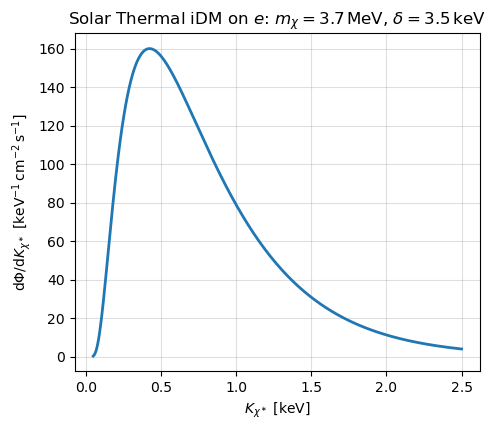
\includegraphics[width=0.5\linewidth]{Differential flux spectra for up-scattering with electrons (fixed delta).png}
    \caption{Spectra of the flux $\Phi$ of $\chi^\ast$ particles up-scattered by electrons per unit kinetic energy $K_{\chi^\ast}$, with $m_\chi = 3.7 \; \text{MeV}$ and $\delta = 3.5 \; \text{keV}$.}
    \label{fig:placeholder}
\end{figure}

\begin{figure}[H]
    \centering
    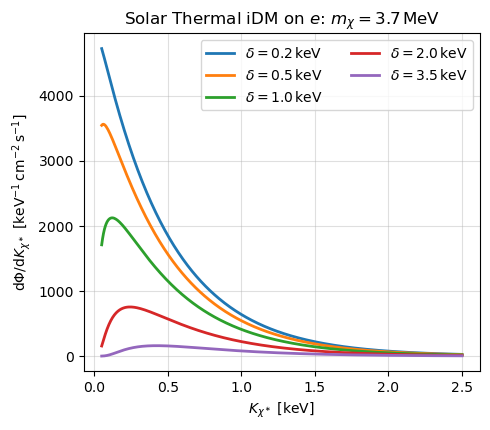
\includegraphics[width=0.5\linewidth]{Differential flux spectra for up-scattering with electrons (changing delta).png}
    \caption{Spectra of the flux $\Phi$ of $\chi^\ast$ particles up-scattered by electrons per unit kinetic energy $K_{\chi^\ast}$, with $m_\chi = 3.7 \; \text{MeV}$ for different values of $\delta \sim \text{keV}$.}
    \label{fig:placeholder}
\end{figure}


\subsection{Up-scattered by nuclei}

For upscattering on nuclei (or free nucleons) the result is obtained by the replacements $e\to T$ (target), $m_e\to m_T$, $\mu_{\chi e}\to \mu_{\chi T}\equiv m_\chi m_T/(m_\chi+m_T)$, $n_e\to n_T$, and $\sigma_e\to\sigma_T$ in the expressions used for electrons. The kinematics is unchanged apart from the reduced mass, so the minimum target speed needed to produce an outgoing state with kinetic energy $K_{\chi^\ast}$ is
\[
v_{\min, T}(K_{\chi^\ast})
=\frac{1}{\sqrt{2m_\chi K_{\chi^\ast}}}\left(\frac{m_\chi K_{\chi^\ast}}{\mu_{\chi T}}+\delta\right),
\qquad q^2\simeq 2m_\chi K_{\chi^\ast}.
\]
Thermally averaging over the Maxwell–Boltzmann distribution at the solar temperature $T_\odot$, the NR differential cross section that enters the flux reads
\[
\Big\langle \frac{d\sigma_{\chi T\to \chi^\ast T}}{dK_{\chi^\ast}}\,v_T \Big\rangle
=\frac{\sigma_T\,m_\chi}{2\,\mu_{\chi T}^2}\,
\sqrt{\frac{2}{\pi}}\sqrt{\frac{m_T}{T_\odot}}\,
\exp\!\left[-\frac{m_T\,v_{\min}^2(K_{\chi^\ast})}{2T_\odot}\right]\,
F_{\rm DM}^2(q)\,F_T^2(q).
\]
For the heavy–mediator limit and pointlike targets (since the Sun is mostly composed of H and He nuclei, it results a good approximation), one may set $F_{\rm DM}(q)\simeq F_T(q)\simeq 1$. The differential flux at Earth from a given target population $T$ is then
\[
\frac{d\Phi_T}{dK_{\chi^\ast}}
= n_T\,
\Big\langle \frac{d\sigma_{\chi T\to \chi^\ast T}}{dK_{\chi^\ast}}\,v_T \Big\rangle\,
\frac{n_{\chi,\odot}\,V_\odot}{4\pi\,(1~\mathrm{AU})^2},
\]
and the total flux is the sum over species, $d\Phi/dK_{\chi^\ast}=\sum_T d\Phi_T/dK_{\chi^\ast}$. For a dark–photon mediator in the contact limit the normalization relates simply to the electron case:
\[
 \bar\sigma_T
\equiv \frac{(g_\chi g_T^{\rm eff})^2\,\mu_{\chi T}^2}{\pi\,(m_{A'}^2+q_{\rm ref}^2)^2}
\simeq \bar\sigma_e\,\frac{\mu_{\chi T}^2}{\mu_{\chi e}^2}\,Z_T^{\,2},
\]
with \(Z_T=1\) for protons and \(Z_T=2\) for \(^4\)He. 

\noindent
Then, the total differential flux is the sum
\[
\boxed{
\frac{d\Phi}{dK_{\chi^\ast}}
=
\frac{\bar\sigma_e\,m_\chi}{2\,\mu_{\chi e}^2}\;
\frac{n_{\chi,\odot}\,V_\odot}{4\pi\,(\mathrm{AU})^2}\;
\left[
n_p\,\sqrt{\frac{2}{\pi}}\sqrt{\frac{m_p}{T_\odot}}\,
e^{-\frac{m_p\,v_{\min,p}^2(K_{\chi^\ast})}{2T_\odot}}
\;+\;
4\,n_{\mathrm{He}}\,\sqrt{\frac{2}{\pi}}\sqrt{\frac{m_{\mathrm{He}}}{T_\odot}}\,
e^{-\frac{m_{\mathrm{He}}\,v_{\min,\mathrm{He}}^2(K_{\chi^\ast})}{2T_\odot}}
\right]
}\; ,
\]

or expressing everything in terms of the electron density and a composition ratio $r\equiv n_{\mathrm{He}}/n_p$ (appropriate for a fully ionized plasma where $n_e=n_p+2n_{\mathrm{He}}$), we have
\[
n_p=\frac{n_e}{1+2r},\qquad n_{\mathrm{He}}=\frac{r\,n_e}{1+2r},
\]
so that
\[
\boxed{
\frac{d\Phi}{dK_{\chi^\ast}}
=
\frac{\sigma_e\,m_\chi}{2\,\mu_{\chi e}^2}\;
\frac{n_{\chi,\odot}\,V_\odot}{4\pi\,(\mathrm{AU})^2}\;
\frac{n_e}{1+2r}\left[
\sqrt{\frac{2}{\pi}}\sqrt{\frac{m_p}{T_\odot}}\,
e^{-\frac{m_p\,v_{\min,p}^2}{2T_\odot}}
\;+\;
4r\,\sqrt{\frac{2}{\pi}}\sqrt{\frac{m_{\mathrm{He}}}{T_\odot}}\,
e^{-\frac{m_{\mathrm{He}}\,v_{\min,\mathrm{He}}^2}{2T_\odot}}
\right]
}\; .
\]

\begin{figure}[H]
    \centering
    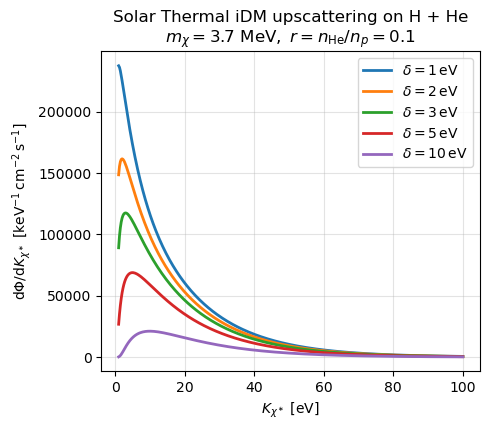
\includegraphics[width=0.5\linewidth]{Differential flux spectra for up-scattering with nuclei.png}
    \caption{Spectra of the flux $\Phi$ of $\chi^\ast$ particles up-scattered by H and He nuclei per unit kinetic energy $K_{\chi^\ast}$, with $m_\chi = 3.7 \; \text{MeV}$ for different values of $\delta \sim \text{keV}$.}
    \label{fig:placeholder}
\end{figure}

\subsection{An important consideration: relative velocity of DM}

In the electron case we worked in the plasma frame and neglected the DM speed, since $v_\chi \ll v_{e}$ in the solar core. For nuclei this approximation generally fails: proton and helium thermal speeds are $\mathcal{O}(10^2\!-\!10^3)\,{\rm km\,s^{-1}}$, comparable to the focused DM speeds $v_\chi\sim v_{\rm esc}$, so the relative speed is controlled by both the DM and the target motions. 

We now include the motion of both populations and average the differential cross section over both the target speed $v_T$ and the DM speed $v_\chi$, following the same steps as in the electron case. The clean, Galilean–invariant starting point is the $q$–differential kernel,
\[
\Big\langle v_{\rm rel}\,\frac{d\sigma_{\chi T\to\chi^\ast T}}{dq^{2}}\Big\rangle
=\int d^3 v_\chi\, f_\chi(\mathbf v_\chi)\int d^3 v_T\, f_T(\mathbf v_T)\;
v_{\rm rel}\,\frac{d\sigma_{\chi T\to\chi^\ast T}}{dq^{2}}(v_{\rm rel}),
\qquad v_{\rm rel}=|\mathbf v_\chi-\mathbf v_T|,
\]
with, in the contact NR limit (replace $e\to T$ and $v_e\to v_{\rm rel}$),
\[
\frac{d\sigma_{\chi T\to\chi^\ast T}}{dq^{2}}(v_{\rm rel})
=\frac{\sigma_T}{2\,\mu_{\chi T}^2}\,
\frac{1}{v_{\rm rel}^{\,2}}\,
\Theta\!\big(v_{\rm rel}-v_{\min,T}(q)\big),
\qquad
v_{\min,T}(q)=\frac{q}{2\mu_{\chi T}}+\frac{\delta}{q}\, .
\]

Targets are taken isotropic Maxwell–Boltzmann in the plasma frame,
\[
f_T(\mathbf v_T)=\left(\frac{m_T}{2\pi T_\odot}\right)^{\!3/2}\!
\exp\!\Big[-\frac{m_T v_T^2}{2T_\odot}\Big],
\]
while for DM we adopt the standard shifted and truncated halo distribution in the Sun’s rest frame,
\[
f_\chi^\odot(\mathbf v_\chi)=
\frac{1}{N_{\rm esc}\,(\pi v_0^2)^{3/2}}
\exp\!\left[-\frac{|\mathbf v_\chi+\mathbf v_\odot|^2}{v_0^2}\right]\,
\Theta\!\big(v_{\rm esc}^{\rm gal}-|\mathbf v_\chi+\mathbf v_\odot|\big),
\quad
N_{\rm esc}=\erf z-\frac{2z}{\sqrt{\pi}}\,e^{-z^2},\ z\equiv \frac{v_{\rm esc}^{\rm gal}}{v_0}.
\]
With this choice the relative–speed distribution of a drifted and a zero–drift Maxwellian is the non-central Maxwell with effective width
\[
s_{\rm rel}^2=s_T^2+s_\chi^2,\qquad 
s_T^2\equiv \frac{T_\odot}{m_T},\qquad
s_\chi^2=\frac{v_0^2}{2},
\]
namely
\[
g(v)\equiv\int d^3v_\chi d^3v_T\,f_\chi^\odot f_T\,\delta\!\big(v-|\mathbf v_\chi-\mathbf v_T|\big)
=\sqrt{\frac{2}{\pi}}\;\frac{v}{s_{\rm rel}\,v_\odot}\,
\sinh\!\Big(\frac{v\,v_\odot}{s_{\rm rel}^2}\Big)\,
\exp\!\Big[-\frac{v^2+v_\odot^2}{2s_{\rm rel}^2}\Big],\qquad 
\int_0^\infty\!dv\,g(v)=1.
\]
Therefore,
\[
\Big\langle v_{\rm rel}\,\frac{d\sigma}{dq^{2}}\Big\rangle
=\frac{\sigma_T}{2\,\mu_{\chi T}^2}\int_{v_{\min,T}(q)}^\infty\!dv\;g(v)\,\frac{1}{v}
=\frac{\sigma_T}{2\,\mu_{\chi T}^2}\;\frac{1}{2v_\odot}\!
\left[
\erf\!\Big(\frac{v_{\min,T}(q)+v_\odot}{\sqrt{2}\,s_{\rm rel}}\Big)
-\erf\!\Big(\frac{v_{\min,T}(q)-v_\odot}{\sqrt{2}\,s_{\rm rel}}\Big)
\right].
\]
In the limit $v_\odot\to 0$ this reduces to the zero–drift result:
\[
\Big\langle v_{\rm rel}\,\frac{d\sigma}{dq^{2}}\Big\rangle
\;\longrightarrow\;
\frac{\sigma_T}{2\,\mu_{\chi T}^2}\,
\sqrt{\frac{2}{\pi}}\;\frac{1}{s_{\rm rel}}\;
\exp\!\left[-\,\frac{v_{\min,T}^2(q)}{2\,s_{\rm rel}^2}\right].
\]

The corresponding differential flux at Earth is obtained by inserting the averaged kernel in the same geometric factor used previously:
\[
\frac{d\Phi_T}{dq^{2}}
= n_T\,
\Big\langle v_{\rm rel}\,\frac{d\sigma_{\chi T\to\chi^\ast T}}{dq^{2}}\Big\rangle
\frac{n_{\chi,\odot}\,V_\odot}{4\pi\,(\mathrm{AU})^2},
\qquad
\frac{d\Phi}{dq^{2}}=\sum_{T=p,\mathrm{He}}\frac{d\Phi_T}{dq^{2}}.
\]

\section{Parameter spaces}

\section{Gravitational effects}

For contact DM–electron scattering, Ref.~[ANPPR, Sec.~III] derives the single–scatter kernel
\begin{equation}
    \label{eq:anppr-kernel}
    \frac{d\Gamma_\chi}{dq\,d\cos\theta_q}
    =\mathcal N\,q\,
    \exp\!\left[
    -\frac{1}{2m_e T}
    \bigg(\frac{m_e}{2m_\chi}(2k_1\cos\theta_q+q)+\frac{q}{2}\bigg)^{\!2}
    \right],
\end{equation}
where $k_1=m_\chi v_\chi$ is the incoming DM momentum in the plasma frame, $q\equiv|\mathbf q|$ the momentum transfer, and $\theta_q$ the angle between $\mathbf k_1$ and $\mathbf q$. The outgoing DM momentum is $\mathbf k_2=\mathbf k_1-\mathbf q$, hence the final speed in the plasma frame is
\begin{equation*}
    \label{eq:v-of-q}
    v \equiv \frac{|\mathbf k_2|}{m_\chi}
    =\frac{1}{m_\chi}\sqrt{k_1^2+q^2-2k_1 q\cos\theta_q}\;.
\end{equation*}
To obtain the spectrum in the outgoing speed $v$, we insert a delta function that enforces
the kinematic relation~\eqref{eq:v-of-q} and integrate over $\cos\theta_q$:
\begin{align}
    \frac{d\Gamma}{dv}
    &=\int_0^\infty\!dq\!\int_{-1}^{1}\!d\cos\theta_q\;
      \frac{d\Gamma_\chi}{dq\,d\cos\theta_q}\,
      \delta\!\left( v-\frac{1}{m_\chi}\sqrt{k_1^2+q^2-2k_1 q\cos\theta_q}\right).
      \label{eq:proj}
\end{align}
Define $c\equiv\cos\theta_q$ and
\[
   g(c;q)\equiv \frac{1}{m_\chi}\sqrt{k_1^2+q^2-2k_1 q\,c}\, .
\]
The root of $v-g(c;q)=0$ is
\begin{equation*}
    \label{eq:costhstar}
    c^\star(v,q)=\frac{k_1^2+q^2-m_\chi^2 v^2}{2k_1 q}\, .
\end{equation*}
Using the identity $\delta[f(c)]=\sum_i \delta(c-c_i)/|f'(c_i)|$ with $f(c)=v-g(c;q)$,
we need the derivative
\begin{align*}
   \frac{dv}{dc}
   &=\frac{d}{dc}\Big[\tfrac{1}{m_\chi}\sqrt{k_1^2+q^2-2k_1 q\,c}\Big]
     = -\,\frac{k_1 q}{m_\chi^2\,v}\,,
\end{align*}
so that the Jacobian is
\begin{equation*}
   \label{eq:jac}
   \left|\frac{dc}{dv}\right|=\frac{m_\chi^2\,v}{k_1\,q}\,.
\end{equation*}
The delta function therefore collapses the angular integral to the value at $c=c^\star(v,q)$,
with $|c^\star|\le 1$. The latter condition is equivalent to the triangle window
\begin{equation*}
   \label{eq:triangle-window}
   |k_1-m_\chi v|\ \le\ q\ \le\ k_1+m_\chi v .
\end{equation*}
Solving the $\cos\theta_q$ integral in~\eqref{eq:proj} yields
\begin{equation*}
    \label{eq:dGdv-from-ANPPR}
    \frac{d\Gamma}{dv}
    =\frac{m_\chi^2 v}{k_1}
     \int_{|k_1-m_\chi v|}^{k_1+m_\chi v}\frac{dq}{q}\;
     \left.\frac{d\Gamma_\chi}{dq\,d\cos\theta_q}\right|_{\cos\theta_q=c^\star(v,q)} .
\end{equation*}
For a contact interaction the explicit factor $q$ in~\eqref{eq:anppr-kernel} cancels the $1/q$
from the Jacobian in~\eqref{eq:dGdv-from-ANPPR}, leaving a one–dimensional Gaussian integral in $q$.
(For endothermic inelastic scattering with splitting $\delta>0$, the projection is unchanged; the only
modification is the inelastic shift in the ANPPR kernel, $q/2\to q/2 + m_e\delta/q$, inside the square bracket.)
Finally, integrating~\eqref{eq:dGdv-from-ANPPR} over $v$ reproduces the total single–scatter rate
$\Gamma_\chi(r)=\int dv\,d\Gamma/dv$, which fixes the overall normalization $\mathcal N$ used in
Eq.~\eqref{eq:anppr-kernel}.

\medskip
\noindent\textbf{Why $d\Gamma/dv$ equals $R_i(w\!\to\! v)$.}
Ref.~[GPR, App.~A] defines the \emph{final–speed–differential} single–scatter rate off target $i$ as
\begin{equation}
    \label{eq:R-def}
    R_i(w\!\to\! v)
    =\int d^3u\, n_i(r)\,f_i(\mathbf u,r)\;
    \underbrace{|\mathbf w-\mathbf u|}_{v_{\rm rel}}\;
    \frac{d\sigma_i}{dv}(v\,|\,w,\mathbf u)\;,
\end{equation}
where $w=v_\chi$ is the incoming DM speed in the plasma frame and $f_i$ is the MB velocity distribution of targets. For an $s$–wave contact interaction the scattering is isotropic in the center–of–mass (CM), and one finds the simple CM\,$\to$\,lab Jacobian
\begin{equation}
    \label{eq:dsigdv-contact}
    \frac{d\sigma_i}{dv}(v\,|\,w,V)
    =\frac{\sigma_{i}}{2}\,\frac{v}{V\,w}\;
    \Theta\!\big(v-|V-w|\big)\,
    \Theta\!\big((V+w)-v\big),
\end{equation}
with $V\equiv|\mathbf V|=|m_\chi\mathbf v_\chi+m_i\mathbf u|/(m_\chi+m_i)$ the CM speed in the plasma frame. Plugging \eqref{eq:dsigdv-contact} into \eqref{eq:R-def} and performing the thermal average over $f_i$ yields $R_i(w\!\to\! v)$.

Now, Eq.~\eqref{eq:dGdv-from-ANPPR} is nothing but a \emph{change of variables} of the very same collision integral: ANPPR first trades the target velocities $\mathbf u$ for the momentum transfer $\mathbf q$, uses the energy–conserving $\delta$–function to do the angle integral, and arrives at the closed kernel \eqref{eq:anppr-kernel}; we have then projected it back to the final speed $v$ with the Jacobian \eqref{eq:costhstar}. Consequently
\begin{equation}[box=\fbox]{equation*}
    \left.\frac{d\Gamma}{dv}\right|_{\text{ANPPR}}
    \equiv R_e(w\!\to\! v)\quad\text{(here $i=e$),}
\end{equation}
provided the same $T(r)$ and $n_e(r)$ are used. This equivalence is also visible when integrating over $v$: starting from ANPPR’s total rate
\begin{equation}
    \label{eq:Gamma-total}
    \Gamma_{\chi-e}(r,v_\chi)
    =\sigma_{\rm tot}\,n_e(r)\,\big\langle v_{\rm rel}\big\rangle
    =\sigma_{\rm tot}\,n_e(r)\,v_\chi\sqrt{\frac{T}{m_e}}\,
    \underbrace{\sqrt{\frac{1}{2\pi}}\!\left[2e^{-x_\chi^2/2}
    +\sqrt{2\pi}\,(1+x_\chi^2)\,\mathrm{erf}\!\left(\frac{x_\chi}{\sqrt2}\right)\right]}_{F(x_\chi)}
    \!,
\end{equation}
with $x_\chi\equiv v_\chi/\sqrt{T/m_e}$, one has by definition
\begin{equation}
    \Gamma_{\chi-e}(r,v_\chi)=\int_0^\infty\!dv\;R_e(w\!=\!v_\chi\!\to\! v)\;,
\end{equation}
i.e.\ both formalisms compute the same thermal average $\langle\sigma v_{\rm rel}\rangle$ but with different choices of variables and order of integration.

\medskip
\noindent\textbf{Imposing the escape condition analytically.}
The Sun’s gravity removes all up–scattered DM with final \emph{plasma–frame} speed below the local escape speed. Therefore, in a shell at radius $r$ we impose
\begin{equation}
    v\ge v_{\rm esc}(r)\qquad\Longrightarrow\qquad
    \left.\frac{d\Gamma}{dv}\right|_{\rm esc}
    =\Theta\!\big(v-v_{\rm esc}(r)\big)\,\frac{d\Gamma}{dv}.
\end{equation}
Equivalently, the escape \emph{rate} in that shell is the $v$–integral above the threshold,
\begin{equation}
    \label{eq:Gamma-esc}
    \Gamma_{\rm esc}(r,v_\chi)
    =\int_{v_{\rm esc}(r)}^\infty\!dv\;R_e(w\!\to\! v)
    =\int_{v_{\rm esc}(r)}^\infty\!dv\;\frac{d\Gamma}{dv}.
\end{equation}
For the contact case the $v$–integral can be evaluated in closed form already \emph{before} the thermal average, which is useful for intuition. Using the kinematic relation
\(
    v^2 = V^2 + u_\ast^2 + 2 V u_\ast\cos\theta^\ast
\)
with $u_\ast=w$ (elastic) and the isotropy of $\cos\theta^\ast$, one finds the speed–differential cross section
\[
    \frac{d\sigma}{dv}=\frac{\sigma_{\rm tot}}{2}\frac{v}{Vw}\,
    \Theta\big(v\in[|V-w|,V+w]\big),
\]
whence, integrating from $v_{\rm cut}\equiv\max\{v_{\rm esc}(r),\,|V-w|\}$ to $V+w$,
\begin{equation}
    \label{eq:Gammaesc-closed}
    \Gamma_{\rm esc}(r\,|\,w,V)
    = n_e f_e\, w\!\int_{v_{\rm cut}}^{V+w}\!dv\,\frac{\sigma_{\rm tot}}{2}\frac{v}{Vw}
    = n_e f_e\,\frac{\sigma_{\rm tot}}{4V}\,
    \Big[(V+w)^2-v_{\rm cut}^2\Big]_+,
\end{equation}
where $[x]_+\equiv x\,\Theta(x)$. The thermal average over $f_e$ then reproduces \eqref{eq:Gamma-esc}.

\medskip
\noindent\textbf{From escaping rates to the flux at the Earth.}
Once the escape condition is imposed, we need to (i) average over the incoming DM and target velocities in each shell, (ii) integrate over production radius, and (iii) dilute the outgoing flux to 1 AU while accounting for the gravitational potential drop between the solar surface and the Earth’s orbit.

First, for any quantity $\mathcal Q$ that depends on $(\mathbf v_\chi,\mathbf u)$ we use the joint average
\(
\langle\mathcal Q\rangle_r
=\int d^3v_\chi\,f_\chi(\mathbf v_\chi)\int d^3u\,f_e(\mathbf u,r)\,\mathcal Q
\),
with $f_\chi$ the DM distribution in the solar frame (typically a shifted Maxwellian). The \emph{escaping} speed spectrum produced in a shell is therefore
\begin{equation}
    \label{eq:shell-spectrum}
    \Big\langle \Big.\frac{d\Gamma}{dv}\Big|_{\rm esc}\Big\rangle_r
    =\int d^3v_\chi\,f_\chi\int d^3u\,f_e\;
    v_{\rm rel}\;\frac{d\sigma}{dv}(v|w,V)\,\Theta\!\big(v-v_{\rm esc}(r)\big)
    \equiv \langle\sigma v_{\rm rel}\rangle_{v\text{-diff},\,r}.
\end{equation}
Second, integrating \eqref{eq:shell-spectrum} over radius and dividing by the area of the sphere at 1 AU gives the differential \emph{surface} flux transported to 1 AU \emph{at the same kinematic label}. If we keep the label as the \emph{final speed at the solar surface} $v_{\odot}$, then pure energy conservation between $R_\odot$ and 1 AU implies
\begin{equation}
    \label{eq:map-v-to-vAU}
    v^2_{\rm AU}=v_{\odot}^2-\big[v_{\rm esc}^2(R_\odot)-v_{\rm esc}^2(\mathrm{AU})\big]
    \equiv v_{\odot}^2-\Delta v_{\rm esc}^2,
    \qquad
    \frac{d v_{\rm AU}}{dv_{\odot}}=\frac{v_{\odot}}{v_{\rm AU}}.
\end{equation}
If instead the observable is the \emph{energy} at 1 AU, $E=\tfrac12 m_\chi v_{\rm AU}^2$, then $dE=m_\chi v_{\rm AU}\,dv_{\rm AU}$ and \eqref{eq:map-v-to-vAU} implies the simple Jacobian
\begin{equation}
    \label{eq:Jac-E}
    \frac{d\Phi}{dE}\Big|_{\rm AU}
    =\frac{1}{m_\chi v_\odot}\,\frac{d\Phi}{dv_\odot}\Big|_{R_\odot}\,,
    \qquad
    v_\odot=\sqrt{v_{\rm AU}^2+\Delta v_{\rm esc}^2}.
\end{equation}
Putting the pieces together, the flux per unit $v_\odot$ at the surface that reaches the Earth is
\begin{equation}[box=\fbox]{equation}
    \label{eq:flux-at-surface}
    \frac{d\Phi}{dv_\odot}
    =\frac{1}{4\pi\,\mathrm{AU}^2}\int_0^{R_\odot}\!4\pi r^2dr\;
    \Big\langle \Big.\frac{d\Gamma}{dv}\Big|_{\rm esc}\Big\rangle_r,
\end{equation}
and the corresponding flux per unit energy at 1 AU follows from \eqref{eq:Jac-E}. In the notation of ANPPR, one often collects the outcome of the radial and velocity averages into a normalized energy distribution $F_{A_\rho}(E)$ for particles that cross the ``impact disc'' of area $A_\rho=\pi(4R_\odot)^2$, and writes the observed flux simply as
\begin{equation}
    \label{eq:geom-flux}
    \frac{d\Phi_{\rm reflected}}{dE}
    =\Phi_{\rm halo}\times \frac{A_\rho}{4\pi\,\mathrm{AU}^2}\;F_{A_\rho}(E)\,,
\end{equation}
where $\Phi_{\rm halo}$ is the incident halo flux. When $F_{A_\rho}$ is plotted as a \emph{shape} (unit–normalized), the total reflected fraction $\eta_{\rm refl}=\int dE\,F_{A_\rho}(E)$ should be reinstated in \eqref{eq:geom-flux}.


\section{Direct detection}

\end{document}